\begin{lemma}
Soit $n \in \setNaturalNumbers$ tel que $n \ge 3$, alors il existe un nombre entre $n$ et $n^2$ (exclus) qui est un carré parfait. 
\end{lemma}

\begin{proof}
Soit $n \in \setNaturalNumbers$ tel que $n \ge 3$, alors
\[
n^2 - 3n = \underbrace{n}_{\ge 0} \underbrace{(n- 3)}_{\ge 0} \ge 0
\]
Donc $n^2 - 3n + 1 > 0$, c'est à dire que $n^2 - 2n + 1 > n$, i.e. $(n-1)^2 > n$. La fonction carré étant croissante sur les nombres strictement positifs, on a de plus $(n-1)^2 < n^2$. Ainsi, 
\[
n < (n-1)^2 < n^2
\]
On a donc trouvé un carré parfait qui appartient à l'intervalle $\integerIntervalOO{n}{n^2}$.
\end{proof}

\begin{lemma}
Soient $n, p\in \setNaturalNumbers$ tels que $p \ge 1$ et $n >
\left\{
\begin{array}{l l}
3 &\text{ si }  p = 1\\
2 &\text{ si }  1 < p \le 10\\
1 &\text{ sinon}\\
\end{array} 
\right.$\\
alors il existe un nombre entre $np$ et $(np)^2$ (exclus) qui est un carré parfait et qui est multiple de $p$. 
\end{lemma}

\begin{proof}
Soient $n, p\in \setNaturalNumbers$ tels que $p \ge 1$ et $n > \dfrac{2}{p}$, alors
\[
\begin{aligned}
(p(n-1))^2 - (np) 
&= (pn)^2 - \left(p + \dfrac{1}{2}\right)2(np) + p^2 \\
&= \left(np - \left(p + \dfrac{1}{2}\right)\right)^2 + p^2 - \left(p + \dfrac{1}{2}\right)^2\\
&= \left(np - \left(p + \dfrac{1}{2}\right)\right)^2 - \dfrac{1}{4} - 2p
\end{aligned}
\]
Donc $(p(n-1))^2 - (np)$ est strictement positif pour $np > p + \dfrac{1}{2} + \sqrt{\dfrac{1}{4} + 2p}$, i.e. $n > 1 + \dfrac{1}{p}\left(\dfrac{1}{2} + \dfrac{1}{2}\sqrt{1 + 8p}\right)$. D'où finalement :
\[
n > 1 + \dfrac{1}{2p}\left(1 + \sqrt{1 + 8p}\right)
\]

D'après le tableau de valeurs de la figure \ref{graphef}, on a 3 cas :
\begin{itemize}
\item $n > 3$ si $p = 1$
\item $n > 2$ si $p \in \integerIntervalCC{2}{3}$
\item $n > 1$ sinon car $f > 1$
\end{itemize}

\begin{figure}[!ht]
\begin{minipage}{0.5\textwidth}
\begin{tikzpicture}
	\begin{axis}[
		xlabel=$p$,
		ylabel={$f(p)=\dfrac{1}{2} + \dfrac{1}{2p}(1 + \sqrt{1 + 8p})$},
        %title={Graphe de $f$ en fonction de $p$\Large},
        xmin = 1, xmax = 15,
        ymin = 1, ymax = 3.5,
        xtick={1,2,3,4,5,6, 7, 8, 9, 10, 11, 12, 13, 14, 15},
        ytick = {1, 1.5, 2, 2.5, 3, 3.5},
        ymajorgrids=true,
        xmajorgrids=true,
        grid style=dashed,
        height = 8.5cm
	]
	% use TeX as calculator:
	\addplot[color=blue, very thick, smooth][domain=1:15]{1 + 1/(2*x)*(1 + (1 + 8*x)^(1/2))};
    
	\end{axis}
\end{tikzpicture}
\end{minipage}
\begin{minipage}{0.49\textwidth}
\begin{flushright}
\directlua{
function f(p)
	return 1 + 1/(2*p)*(1 + math.sqrt(1 + 8*p))
end
}
\begin{tabular}{l l}
\hline
p & f(p)\\
\hline
1 & \directlua{tex.sprint(f(1))}\\
2 & \directlua{tex.sprint(f(2))}\\
3 & \directlua{tex.sprint(f(3))}\\
4 & \directlua{tex.sprint(f(4))}\\
5 & \directlua{tex.sprint(f(5))}\\
6 & \directlua{tex.sprint(f(6))}\\
7 & \directlua{tex.sprint(f(7))}\\
8 & \directlua{tex.sprint(f(8))}\\
9 & \directlua{tex.sprint(f(9))}\\
10 & \directlua{tex.sprint(f(10))}\\
11 & \directlua{tex.sprint(f(11))}\\
12 & \directlua{tex.sprint(f(12))}\\
13 & \directlua{tex.sprint(f(13))}\\
14 & \directlua{tex.sprint(f(14))}\\
15 & \directlua{tex.sprint(f(15))}\\
16 & \directlua{tex.sprint(f(16))}\\
\hline
\end{tabular}
\end{flushright}
\end{minipage}
\caption{Graphe et tableau de valeur de $f$ en fonction de $p$}
\label{graphef}
\end{figure}

Le cas $p = 1$ est redondant avec le lemme précédent car tous les nombres sont divisibles par $1$.
\end{proof}
